\section{Introducción}
\subsection{¿Qué es la visión artificial?}
Los seres humanos somos capaces de percibir con facilidad el entorno tridimensional que nos rodea. Durante décadas, el funcionamiento de nuestra visión ha sido fruto de extensivo estudio por parte de psicólogos de la percepción, pero aún no se conoce el funcionamiento de manera exacta  \cite{book:szeliski}.

Paralelamente, los investigadores en visión artificial han desarrollado técnicas matemáticas para, a partir de imágenes, reconstruir la apariencia tridimensional de objetos. Actualmente somos capaces de, entre otras cosas, generar un modelo 3D parcial de un entorno a partir de miles de fotografías solapadas, seguir el movimiento de una persona sobre un fondo complejo y, con moderado éxito, reconocer y nombrar a las personas de una fotografía a partir de características como el pelo, la cara o la ropa. Entre otras aplicaciones más avanzadas se encuentran detectar y clasificar objetos o elaborar descripciones verbales a partir de imágenes o vídeos.

Sin embargo, a pesar de estos avances, hacer que un ordenador sea capaz de interpretar una imagen al mismo nivel que lo haría un niño sigue siendo un sueño sin cumplir. La dificultad del problema que nos ocupa suele ser subestimada, ya que se suele tender a pensar que las partes difíciles de la inteligencia artificial son las cognitivas y no las relativas a la percepción. 

Pero, ¿qué es lo que hace tan difícil la visión por computador? En parte es que, dado nuestro desconocimiento del funcionamiento de nuestra visión, es un \textit{problema inverso}, dada una cantidad insuficiente de información (una imagen o un video), tratamos de llegar a las incógnitas que nos permiten especificar una solución completa. Es decir, a partir de una imagen, tratamos de reconstruir sus propiedades, como las formas, iluminación y color.

Ahora bien, no todo son malas noticias: la visión por computador tiene numerosos casos de uso hoy en día. Entre sus aplicaciones encontramos cosas tan mundanas como (\citeauthor*{book:szeliski}):
\begin{itemize}
\item \textbf{Reconocimiento de caracteres óptico:} Se ha llegado a reconocer caracteres numéricos con una tasa de error del 0.23\% \cite{art:2012arXiv1202.2745C}.
\item \textbf{Inspección mecanizada:} inspección de partes de automóviles o aeronaves a fin de, por ejemplo, encontrar defectos en el metal (Figura \ref{fig:apps1a}).
\item \textbf{Construcción de modelos 3D} construcción automatizada de modelos 3D a partir de fotografías aéreas como las que usa Google Maps (Figura \ref{fig:apps1b}).
\item \textbf{Seguridad en automóviles:} reconocimiento de obstáculos tales como peatones u otros coches, en condiciones en las que el radar o el lidar no funcionan bien, en tecnologías como \href{https://www.mobileye.com/}{Mobileye}.
\item \textbf{Reconocimiento de huellas dactilares y biométricas:} Usado ampliamente hoy en día en teléfonos móviles.
\item \textbf{Reconocimiento y localización de objetos, categorías y acciones:} usando deep learning, se ha conseguido un cierto grado de precisión a la hora de reconocer objetos dispersos en una escena.
\end{itemize}

\begin{figure}
\begin{subfigure}{.5\textwidth}
  \centering
  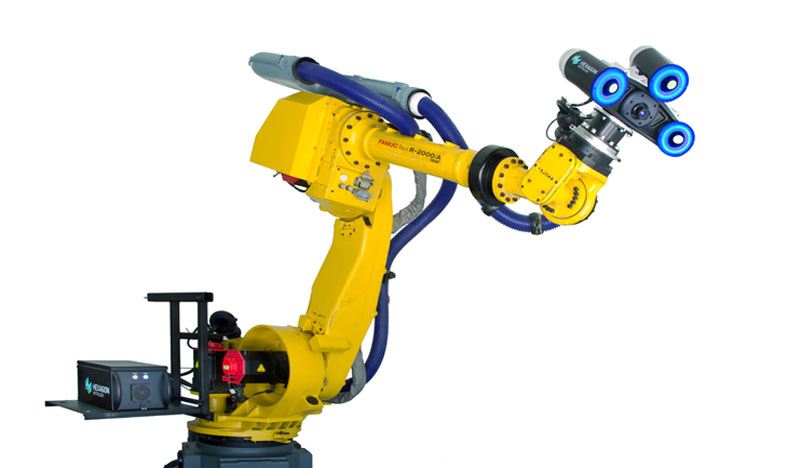
\includegraphics[width=.9\linewidth]{images/camera.jpg}
  \caption { }
  \label{fig:apps1a}
\end{subfigure}%
\begin{subfigure}{.5\textwidth}
  \centering
  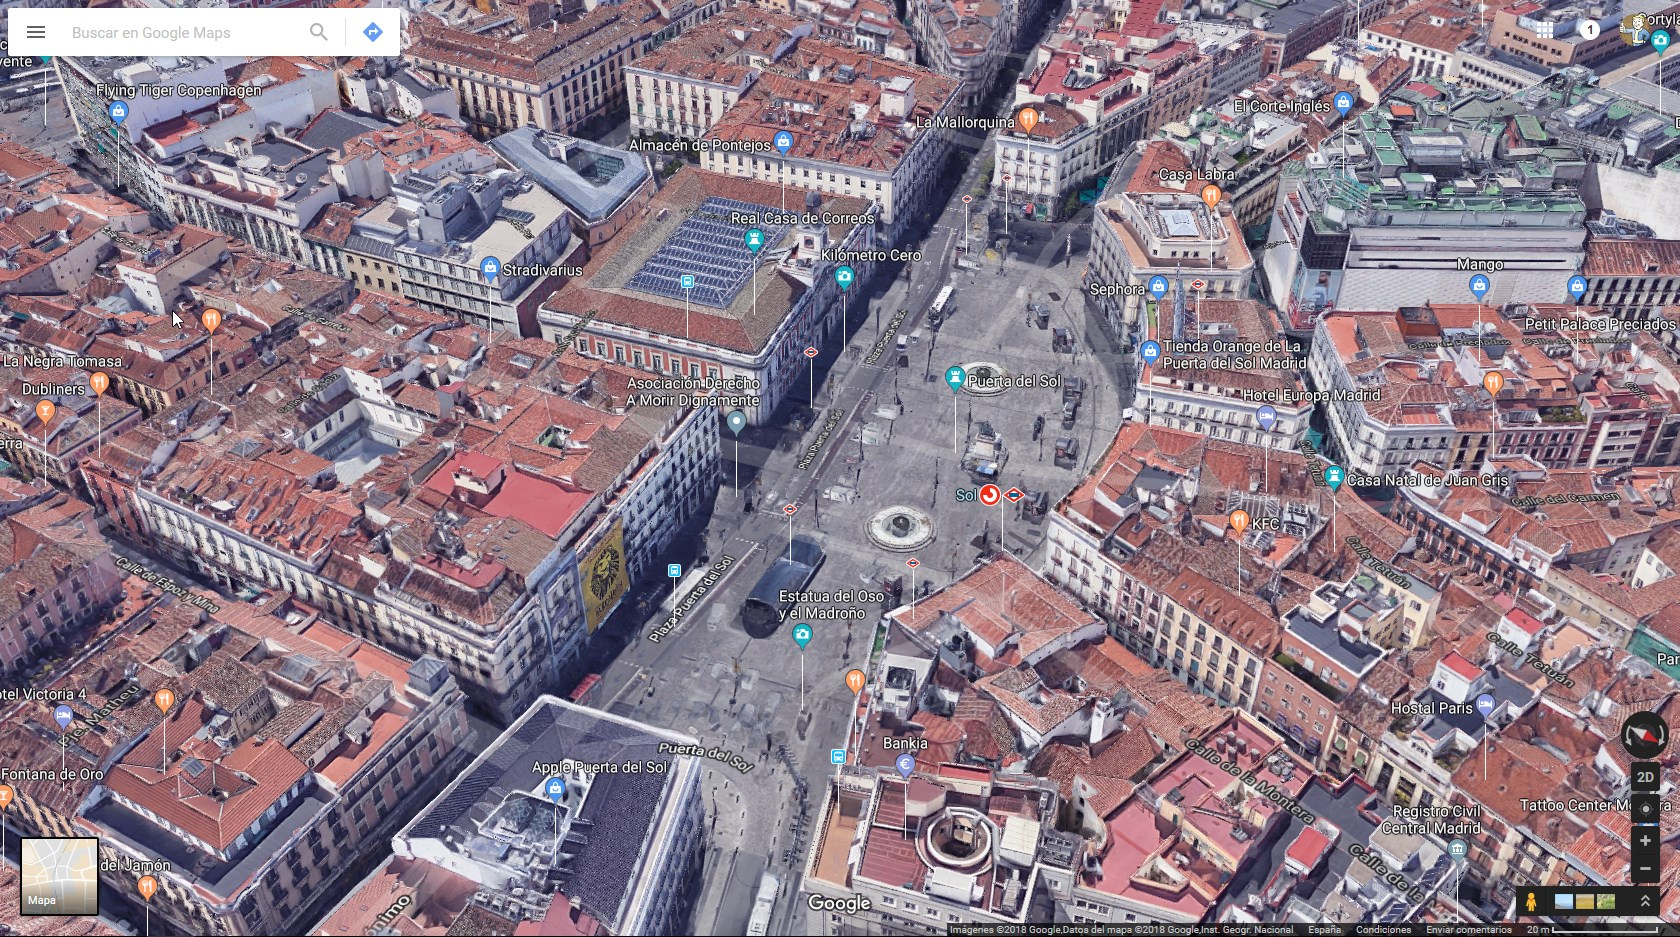
\includegraphics[width=.9\linewidth]{images/maps.jpg}
  \caption { }
  \label{fig:apps1b}
\end{subfigure}
\caption{Algunas aplicaciones de la visión artificial: (a) sistema de digitalizado por luz blanca \href{http://www.hexagonmi.com/es-ES/products/white-light-scanner-systems/hexagon-metrology-wls400a}{WLS400A}. (b) reconstrucción 3D en Google Maps de la Puerta del Sol. }
\label{fig:applications}
\end{figure}

\subsection{Breve historia de la visión artificial}

\begin{figure}[H]
	\centering
	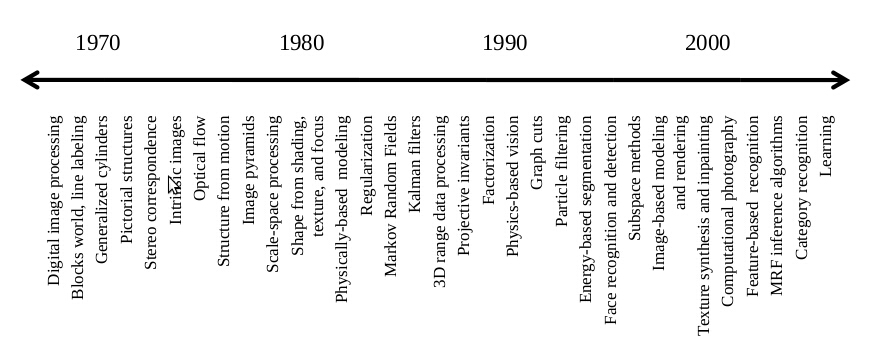
\includegraphics[width=0.8\textwidth]{images/timeline}
	\caption{Timeline de las aportaciones más importantes a la visión artificial \cite{book:szeliski}}
\end{figure}

La investigación en visión artificial comienza en la \textbf{década de los 70}. En esta época, los pioneros en el campo de la IA y la robótica creían que resolver el problema de la entrada visual sería un trabajo fácil hacia la resolución de problemas de mayor envergadura. De hecho, tanto es así, que en 1966 Marvin Minsky le asignó a su alumno en el MIT Gerald Jay Sussman un proyecto de verano que consistía en enlazar una cámara a un ordenador y que este describiera lo que veía.

Lo que distinguió la visión por computador del campo del procesado de imágenes digitales fue la intención de reconstruir la estructura tridimensional del mundo a partir de las imágenes. Los primeros intentos en este sentido estaban relacionados con la extracción de ejes y posterior inferencia de la estructura 3D del objeto.

En la \textbf{década de 1980} los esfuerzos se centraron en técnicas matemáticas mas sofisticadas para el análisis. Empiezan a usarse ampliamente técnicas como las pirámides de imágenes, y continuó la investigación en una mejor detección de bordes y contornos. Comienzan a adoptarse técnicas de detección de formas a partir de sombreado, textura, o enfoque. Posteriormente, algunos investigadores vieron que estas técnicas podían ser generalizadas usando el mismo modelo matemático si se planteaban como problemas de optimización. También aparecieron las primeras redes neuronales aplicadas al campo de la visión por computador.

En la \textbf{década de 1990} continuó la investigación en todo lo anteriormente mencionado, pero algunos de los temas vieron un aumento en su actividad. Hubo un esfuerzo por solucionar el problema de la estructura a partir del movimiento. El trabajo comenzado en la década anterior consistente en usar medidas detalladas de color e intensidad en combinación con modelos físicos precisos acabó por crear su propio subcampo llamado visión basada en la física.

Los algoritmos de tracking mejoraron, incluidos los de tracking por contorno usando contornos activos, así como los basados en intensidad. Normalmente se aplicaron al tracking de caras o de cuerpos completos.

La segmentación de imagen fue un tema de investigación activo, y produjo técnicas como \textit{mean shift}. Comienzan a aparecer técnicas de aprendizaje basadas en la estadística, de las que surgen los primeros algoritmos de reconocimiento de caras.

El avance más notable en esta década fue la interacción con la computación gráfica. La idea de manipular imágenes del mundo real para crear animaciones tomó forma mediante técnicas de \textit{morphing} y se aplicó después a técnicas de interpolación y creación de imágenes panorámicas. A la vez, empezaron a introducirse técnicas consistentes en crear modelos 3D a partir de colecciones de imágenes.

Durante la \textbf{década de los 2000} continuó la interacción entre el campo de la visión y el de los gráficos. Una tendencia de esta década fue la proliferación de técnicas basadas en \textit{features} para el reconocimiento de objetos. Estas técnicas también dominan otras tareas del reconocimiento como el reconocimiento de la escena o de localización.

Otra tendencia, que sigue presente en la actualidad, es la aplicación de técnicas de \textit{machine learning} a problemas de visión artificial, como es el uso de redes neuronales convolucionales. El crecimiento de esta técnica coincide con la gran disponibilidad en Internet de enormes cantidades de datos etiquetados, así como la multiplicación de la capacidad de cómputo, lo que facilitó las tareas de aprendizaje \citep{book:szeliski}.

Al igual que en el campo del \textit{machine learning}, las redes neuronales han cobrado una importancia vital, y se han logrado verdaderamente grandes avances haciendo uso de ellas. Un ejemplo del estado actual del campo es el trabajo de \citet{art:2017arXiv170306870H} que muestra el avance en segmentación de imagen que se ha logrado usando ANN.

También hay avances en la conducción autónoma usando visión por computador, de hecho NVIDIA tiene actualmente en funcionamiento una plataforma para coches autónomos llamada NVIDIA DRIVE. Dicha plataforma, nuevamente, hace uso de técnicas de deep learning para detectar obstáculos, señales, etc.

\begin{figure}
    \centering
    \label{fig:kinect}
    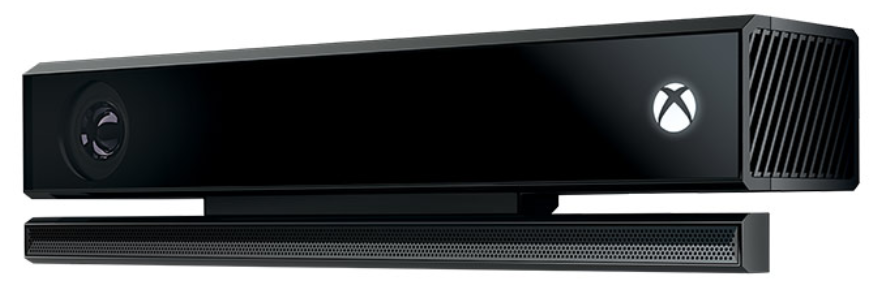
\includegraphics[width=0.7\textwidth]{images/kinect}
    \caption{Imagen promocional de Kinect}
\end{figure}

También existe Kinect, que es un dispositivo cuyo propósito es el de estimar la posición y los gestos del usuario mediante cámaras de profundidad. Kinect surgió en 2010 como un controlador de videojuegos, pero se puede usar para otros propósitos.